\documentclass{article}
\usepackage[a4paper,left=1in, right=1in, top=1in, bottom=1in]{geometry}
\usepackage{hyperref}
\usepackage{graphicx}
\usepackage{wrapfig}
\usepackage{subcaption}
\usepackage{comment}
\usepackage{array}
\usepackage{longtable}
\DeclareGraphicsExtensions{.pdf,.png,.jpg}
\graphicspath{ {./images/} }
\begin{document}
\title{Gibbot v4 PCB}
\author{Andrew Griesemer}
\maketitle
\section{dsPIC Pinout}
\begin{figure}[h!]
	\centering
	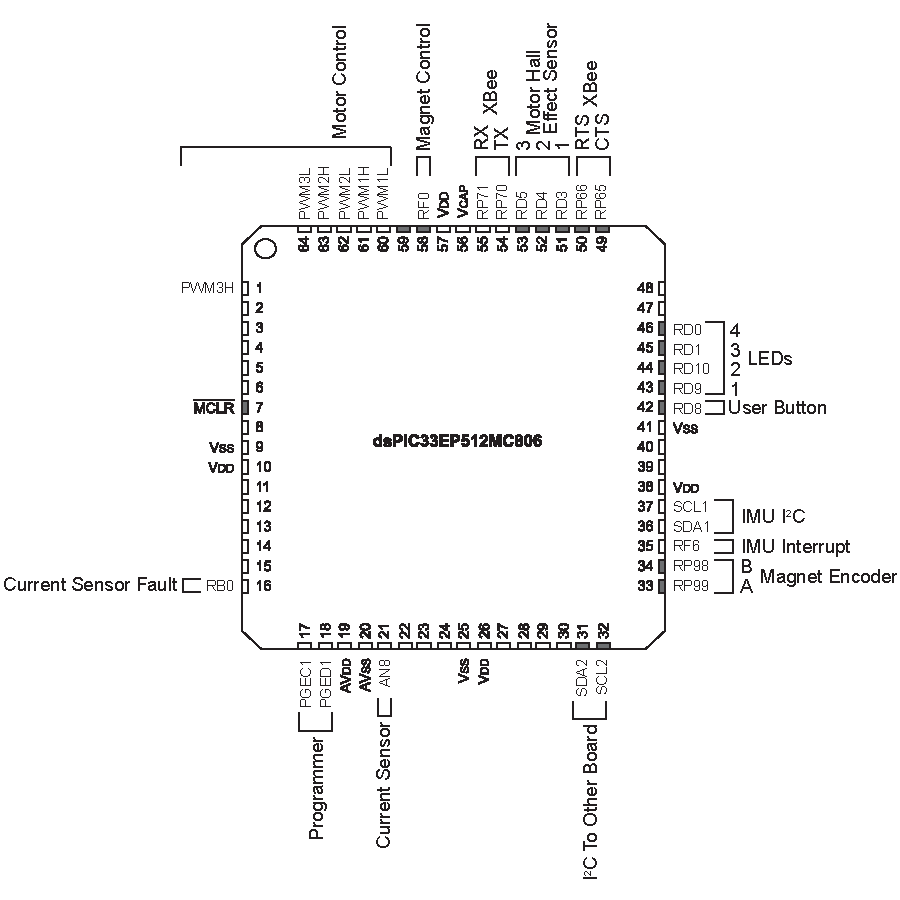
\includegraphics[width=0.8\textwidth, page=1]{breakout}
	\caption{dsPIC Pin Assignments for main board}
	\label{pinout1}
\end{figure}
\begin{figure}[h!]
	\centering
	\includegraphics[width=0.8\textwidth, page=2]{breakout}
	\caption{dsPIC Pin Assignments for secondary board}
	\label{pinout2}
\end{figure}

\section{Power Regulation}
The board is powered by a 24V power cable. 



\begin{longtable}{|c | c | c |  >{\centering\arraybackslash}p{0.4\textwidth} |} 
\hline
Component & Current per unit & Total Component & Value Source\\ \hline
\multicolumn{4}{|l|} {\textbf{5V}}  \\ \hline
2 Encoders & 78mA x 2 & 156mA & 62mA maximum no load current + 8mA x 2 maximum output current\footnote{E3 1600 CPR product page http://www.usdigital.com/products/e3}\\ \hline
\multicolumn{4}{|l|} {\textbf{3.3V}}  \\ \hline
dsPIC && 320mA & Absolute maximum rating current from VSS\footnote{dsPIC33EP512MC806 datasheet http://ww1.microchip.com/downloads/en/DeviceDoc/70616g.pdf}\\ \hline
Status LEDs & 3.3mA x 6& 20mA & Assuming 3.3V and 1k resistor\\ \hline
IMU && 10mA & 3.9mA gyro + 6mA magnetometer\footnote{MPU-9150 datasheet http://dlnmh9ip6v2uc.cloudfront.net/datasheets/Sensors/IMU/PS-MPU-9150A.pdf} \\ \hline
IR LEDs &10mA x 6 & 60 mA & 3.3V  and 330 ohm resistor\\ \hline
\textbf{Total} && \textbf{0.410 A} &\\ \hline
\end{longtable}
\subsection{Digital Isolation}

\section{Inertial Measurement Unit - MPU9150}
The MPU9150 is a 9 axis sensor that draws data from a 3-axis gyroscope, a 3-axis accelerometer and a 3-axis magnetometer. One sensor is attached to each board. Neither sensor has been configured. The supporting circuitry follows is shown in Figure \ref{mpu9150} below \footnote{MPU9150 
Product Specification p21 http://www.invensense.com/mems/gyro/documents/PS-MPU-9150A-00v4\_3.pdf}.

\begin{figure}[h!]
	\centering
	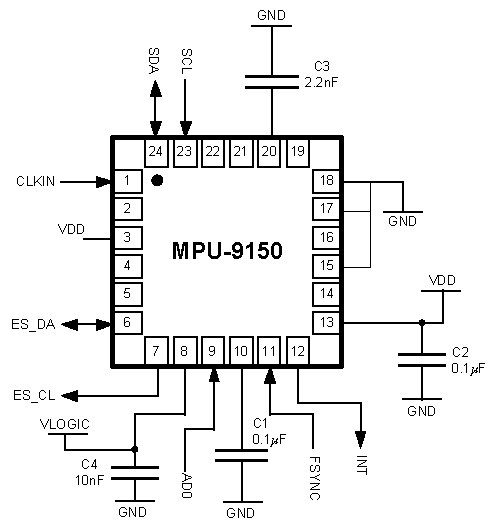
\includegraphics[width=0.4\textwidth]{mpu9150}
	\caption{MPU9150 Typical Operating Circuit}
	\label{mpu9150}
\end{figure}

\textbf{This iteration of the board does not have pull-up resistors on the I\textsuperscript{2}C communication lines that are required for communication between the MPU9150 and the dsPIC.}
\section{XBee}

\section{Magnet Control}

\section{BLDC Motor Driver}
\subsection{BLDC Motor Background}
A Brushless DC Motor is similar to a brushed DC motor except it lacks the internal brushes that allow a typical DC motor to reverse the direction of current flow as the rotor coil rotates within the magnetic stator. In order to drive a BLDC motor the direction of current flow must be commutated by external control circuitry. The benefit of BLDC motor over brushed motor is they tend to be lighter weight for the same amount of torque and they have increased longevity.

A typical BLDC motor has two or more coils and a sensor that can determine the rotational position of the rotor. A microcontroller reads the state of the sensor and changes the direction of current across the coils in order to maximize torque. The BLDC motor on the Gibbot is the Maxon EC 60 Flat which has 3 coils and 3 Hall Effect sensors that detect the rotational position of the rotor. The commutation pattern from the Maxon E-Paper Catalog is shown in Figure \ref{fig:commutation}a and modified for clarity in Figure \ref{fig:commutation}b. 
\begin{figure}[h]
	\centering
	\begin{subfigure}{0.4\textwidth}
		\includegraphics[width=\textwidth]{commutation}
		\caption{}
	\end{subfigure}
	\quad
	\begin{subfigure}{0.4\textwidth}
		\includegraphics[width=\textwidth]{commutation2}
		\caption{}
	\end{subfigure}
	\caption{The commutation pattern for the Maxon EC 60 Flat Motor.\protect\footnotemark}
	\label{fig:commutation}
\end{figure}
\footnotetext{\raggedright Figure \ref{fig:commutation} is taken from pg 32 of the Maxon E-Paper Catalog http://epaper.maxonmotor.ch/en/}

For a lower power application the control of each coil of the motor could be accomplished by a typical H-bridge. Because the Gibbot requires at least 10A at 24V we were forced to create high powe H-bridges from MOSFETs.  Figure~\ref{fig:hbridge} shows the H-bridge configuration for a single coil. 
\begin{figure}[h]
	\centering
	\includegraphics[width=0.3\textwidth]{hbridge}
	\caption{A single H bridge for the BLDC motor}
	\label{fig:hbridge}
\end{figure}

\subsection{HIP4086 Driver}
The driver circuit uses Intersil's HIP4086 3-Phase MOSFET driver\footnote{Datasheet http://www.intersil.com/content/dam/Intersil/documents/hip4/hip4086-a.pdf}. This chip solves two issues with driving the MOSFETs from a dsPIC, (1) stepping up the control voltage for the low side MOSFET from the microcontroller's logic level 3.3V to the 15V required to fully turn on the MOSFET. (2) Because the high side MOSFET's source is connected to the motor coil, the Gate-to-Source voltage must be 15V plus the motor drive voltage to ensure the MOSFET is fully on. The HIP4086 accomplishes this with Bootstrap capacitors (more info in Section \ref{sec:bootstrap}). The chip also has added functionality such as programmable deadtime and a bootstrap capacitor refresh pulse. 

\subsection{MOSFET Selection}
The bridge MOSFETs are the most critical components in the BLDC driver. 
\begin{description}
\item[Max Continuous Current]
The required continuous current for the motor to achieve the desired torque was calculated to be 10A\footnote{WHAT SIMULATION?}. 
\item[Max Drain to Source Voltage ($V_{DS}$)] The required drain-to-source voltage is the same as the Motor Supply Voltage, which was 48V, but is now 24V. To keep the design flexible to the higher voltage range $V_{DS}$ is set a value above 48V. 
\item[Max Gate-to-Source Voltage ($V_{GS}$)] The required gate-to-source voltage is determined by the gate drive voltage of the HIP4086 driver. This gate drive voltage is the same as the supply voltage for the HIP4086. The recommended maximum operating supply voltage on the HIP4086 datasheet\footnote{\raggedright HIP4086 Datasheet pg 5 http://www.intersil.com/content/dam/Intersil/documents/hip4/hip4086-a.pdf} is 15V. To keep the design flexible to supply voltages for the HIP4086 the max gate-to-source voltage should be at least $\pm15V$. 
\item[Gate Charge ($Q_G$)] The turn on speed of the MOSFET is partially determined by the gate charge. The gate charge listed on a datasheet is typically the gate charge at a $V_{GS}= 5V$ . If the HIP4086 has a supply voltage of 15V, in this application $V_{GS}= 15V$ . The appropriate value of $V_{GS}$ can be determined from Figure \ref{fig:qg}. For the configuration 
\begin{figure}[h]
	\begin{subfigure}{0.4\textwidth}
		\includegraphics[width=\textwidth]{qg}
		\caption{}
	\end{subfigure}
	\begin{subfigure}{0.4\textwidth}
		\includegraphics[width=\textwidth]{qg2}
		\caption{}
	\end{subfigure}
	\caption{Typical Gate Charge vs. Gate-to-Source Voltage (a) from the IRFR3806 datasheet \protect\footnotemark~(b) linearly extrapolated to $V_{GS}=15V$.}
	\label{fig:qg} 
\end{figure}
\footnotetext{\raggedright IRFR3806PbF datasheet pg 3 http://www.irf.com/product-info/datasheets/data/irfr3806pbf.pdf}
From the plot, the Gate Charge is 33nC.
\item[On State Drain-to-Source Resistance ($R_{DS(ON)}$)] Should be minimized.
 \item[Maximum Power Dissipation ($P_D$)] This value is not considered in MOSFET selection. While the ability of the MOSFET to dissipate heat from conducting is important, the way in which $P_{D,MAX}$ is defined varies widely between manufacturers. Moreover, the ability of a MOSFET to dissipate heat should not vary significantly between different devices in the same physical package. Determining a specification for power dissipation would also be difficult because it involves a combination of the power dissipated during turn-on and turn-off periods when $R_{DS}$ is high and the power dissipated during the fully on state at the much lower $R_{DS(ON)}$.
\end{description}

\subsection{Clamping Circuit}
\begin{figure}[h]
	\centering
	\begin{subfigure}{0.5\textwidth}
		\includegraphics[width=\textwidth]{clamp1}
		\caption{HIP4086 Datasheet}
	\end{subfigure}
	\quad
	\begin{subfigure}{0.35\textwidth}
		\includegraphics[width=\textwidth]{clamp2}
		\caption{HIP4086 Demo Board User guide}
	\end{subfigure}
	\caption{Alternate clamping circuitry from the HIP4086 documentation\protect\footnotemark.}
	\label{fig:commutation}
\end{figure}
\footnotetext{HIP4086 datasheet pg 12 http://www.intersil.com/content/dam/Intersil/documents/hip4/hip4086-a.pdf and HIP4086 Demo Board User Guide, Application Note 1829 pg 7 http://www.intersil.com/content/dam/Intersil/documents/an18/an1829.pdf}

\subsection{Calculate Required Deadtime}

\subsection{Bootstrap Capacitor, Diode and Resistor Selection}
\label{sec:bootstrap}
The boot capacitor value is chosen not only to supply the internal bias current of the high-side driver but also, and more significantly, to provide the gate charge of the driven FET without causing the boot voltage to sag excessively. In practice, the boot capacitor should have a total charge that is about 20 times the gate charge of the driven power FET for approximately a 5\% drop in voltage after charge has been transferred from the boot capacitor to the gate capacitance.

\[Q_{total} = Q_{gate} + Period * (I_{HB} + I_{GateLeak})\]

\noindent Where:

$Q_{gate}$ = Gate Charge of the MOSFET

$Period$ = On time of the high side MOSFET

$I_{HB}$ = Worst case high side current through the xHB pin of the HIP4086

$I_{GateLeak}$ = Leakage current of the MOSFET gate
\[Q_{total} = 18nC + \frac{1}{20,000Hz}*(100uA + 100 nA) = 23nC\]

\[Cboot = \frac{Q_{total}}{Ripple Voltage}\]
\begin{comment}
From a document by Fairchild Semiconductor on [Design of a Bootstrap Circuit](http://www.fairchildsemi.com/an/AN/AN-6076.pdf):

The bootstrap capacitor (CBOOT) is charged every time the low-side driver is on and the output pin is below the supply voltage (VDD) of the gate driver. The bootstrap capacitor is discharged only when the high-side switch is turned on. This bootstrap capacitor is the supply voltage (VBS) for the high circuit section. The first parameter to take into account is the maximum voltage drop that we have to guarantee when the high-side switch is in on state. The maximum allowable voltage drop (VBOOT) depends on the minimum gate drive voltage (for the high-side switch) to maintain. The capacitor drop must be: 

dVboot = VDD - Vf - Vgsmin

VDD = Supply voltage of gate driver
Vf = Bootstrap diode forward voltage drop
Vgsmin = minimum gate-source voltage

The value of bootstrap capacitor is calculated by:

Cboot = Qtotal / dVboot 

where Qtotal is the total amount of the charge supplied by the capacitor. 

The total charge supplied by the bootstrap capacitor is calculated by:

Qtotal = Qgate + (Ilkgs + Ilkcap + Iggs + Ilk + Ilkdioded)*ton + Qls

Qgate = Total gate charge;
Ilkgs = Switch gate-source leakage current;
Ilkcap = Bootstrap capacitor leakage current;
Iqgs = Bootstrap circuit quiescent current;
Ilk = Bootstrap circuit leakage current;
Ilkdioded = Bootstrap diode leakage current;
ton = High-side switch on time;
Qls = Charge required by the internal level shifter, which is set to 3nC for all HV gate drivers;

For the IRLR024 MOSFETs used in version 1 of the drive circuit:
Qgate = 18nC
Ilkgs = 100nA

For the HIP4086 used in version 1 of the drive circuit:
Iqgs = 50 uA


\end{comment}

\subsection{Set Dead Time on HIP4086}
Because the gate capacitance of the MOSFET keeps the MOSFET on for a period of time after the control signal has gone low, there must be a delay between the turn-off event of one PWM
output in a complementary pair and the turn-on event of the other. Otherwise shoot through might occur when both MOSFETs are conducting causing the power to short to ground. The time between transitions of the control PWM signal is called dead time. In the current configurations of the Gibbot dead time is redudantly programmed into both the dsPIC PWM control as well as the HIP4086. 

Dead time on the HIP4086 is set using a resistor between ground and the pin $R_{DEL}$ on the HIP4086. Figure \ref{fig:deadtime} from the HIP4086 datasheet can be used to set $R_{DEL}$ approximately.
\begin{figure}[h]
	\centering
	\includegraphics[width=0.5\textwidth]{deadtime}
	\caption{ $R_{DEL}$ vs. Dead Time\protect\footnotemark}
	\label{fig:deadtime}
\end{figure}
\footnotetext{\raggedright From HIP4086 3-Phase Bridge Driver Configurations
and Applications pg 4 \href{http://www.intersil.com/content/dam/Intersil/documents/an96/an9642.pdf}{http://www.intersil.com/content/dam/Intersil/documents/an96/an9642.pdf}}

\section{IR LEDs}
The Gibbot is mounted with six \href{http://www.naturalpoint.com/optitrack/static/documents/850\%20nm\%20IR\%20LED\%20Data\%20Sheet.pdf}{Optitrack IR LEDs}.
The LEDs are mounted on the face plate in three clusters (2 above the top magnet, 1 above the motor, 3 above the bottom magnet) so that the Optitrack cameras can detect the position of each magnet and the motor joint. 
\subsection{IR LED Resistor Values}
In this iteration all of the LEDs are powered on 5V lines. The minimum resistor values were calculated as follows:
\begin{description}
\item{1 LED}
\[\frac{5V-(1*V_{F,MAX})}{I_{F,MAX}}=\frac{5V-1.6V}{100mA} = 34\Omega\]
\item{2 LED}
\[\frac{5V-(2*V_{F,MAX})}{I_{F,MAX}}=\frac{5V-3.2V}{100mA} = 18\Omega\]
\item{3 LED}
\[\frac{5V-(3*V_{F,MAX})}{I_{F,MAX}}=\frac{5V-4.8V}{100mA} = 2\Omega\]
\end{description}
Where:

$V_{F,MAX} =1.6V$

$I_{F,MAX} =100mA$\\
To avoid the risk of running maximum current through the resistors these value should be increased by about 50\%.

\section{Current Sensor}
The current sensor used on the board is the
 \href{file:///Users/ajgriesemer/Downloads/ACS716-Datasheet%20(1).pdf}{ACS716KLATR-12CB-T}
which has an optimized accuracy range of +/- 12.5A and a linear sensing range of +/- 37.5A. The sensor outputs an analog voltage proportional to the current through its sensing path, centered at 1.65V for zero current with a slope of 37mV/A.
\subsection{dsPIC ADC Inductor}
The dsPIC33EP512MC806 datasheet\footnote{\raggedright dsPIC33EPXXX(GP/MC/MU)806/810/814 datasheet pg 32 http://ww1.microchip.com/downloads/en/DeviceDoc/70616g.pdf} 
recommends an inductor between the $V_{DD}$ and $A_{VDD}$ to improve ADC noise rejection. The inductance of this inductor is calculated as follows: \[ L = \left(\frac{1}{2*\pi*\frac{F_{CNV}}{2}*\sqrt{C}} \right)^2 = \left(\frac{1}{2*\pi\frac{F_{CNV}}{2}*\sqrt{.1uF}} \right)^2\]
Where: 

$F_{CNV}$ = ADC Conversion Rate

Until the ADC is configured and a conversion rate is determined the inductor should be replaced with a 0ohm resistor. 
\subsection{ACS716 Filter Capacitor}
The ACS716 allows for a filter capacitor to limit noise in the sensor. The capacitance is determined from the plot below. Since the motor is driven with a PWM frequency at 20kHz an appropriate bandwidth is between 10 and 20kHz. The corresponding capacitance from Figure \ref{fig:filter} is between 5 and 9nF.
\begin{figure}[h]
	\centering
	\includegraphics[width=0.5\textwidth]{acs716filter}
	\caption{ACS716 Bandwidth versus External Capacitor Value, $C_F$\protect\footnotemark}
	\label{fig:filter}
\end{figure}
\footnotetext{From ACS716 Datasheet pg 10 http://www.allegromicro.com/\textasciitilde/media/Files/Datasheets/ACS716-Datasheet.ashx} 
\subsection{Overcurrent Threshold}
The overcurrent threshold voltage allows us to detect if the current level is above a user-set limit, likely because of a short. The overcurrent limit is set using a voltage divider composed of $R_H$ and $R_L$ to set a reference voltage on pin $V_{OC}$. When the current through the current path is detected to be higher than 
\[C_{OC} = I_{OC}*37mV/A\] 
the ACS716 drives the output of the FAULT pin high. We chose to set the current threshold at 30A. 
\[C_{OC} = 30A*37mV/A=1.1V\] 
Resistors values of $R_H=2k$ and $R_L=1k$ set $V_{OC}$ at 
\[V_{OC} = 3.3V*\frac{1k}{1k+2k}=1.1V\]
To prevent the fault detection from triggering because of noise a capacitor is connected between fault and ground. The maximum recomended value of 22nF is used.
In previous iterations this features was configured, but the FAULT pin was not connected to the PIC. The pin is now connected to pin B0 on the PIC.

\section{Wire Gages}
\subsection{Wire Sources}
The standard wire gages on purchased connectors are:
\begin{description}
\item[Orbex Slip Ring 2A:]
AWG26 or AWG28
\item[Sparkfun JST PH Jumper Wire:]
24 AWG
\item[Sparkfun JST SH Jumper Wire:]
28 AWG
\item[Mechatronics Lab Red \& Black]
22 AWG
\item[Nick's stores Red, Blue \& Green]
30 AWG
\item[NxR]
30 AWG Black\\
22 AWG Green\\
16-19 AWG Lime Green\\
22 AWG Black, Blue, Red White, Green, Orange in Grey case\\
16 AWG Blue, Brown Green\\
Unknown AWG Red, Black, White shielded clear\\
22 AWG Striped
\end{description}
\subsection{Wire Requirements}
\textbf{24V Power}\\
\textbf{Current Sensor}\\
\textbf{Main Board 5V Power} 22 AWG Red \& Black\\
\textbf{Secondary Board 5V Power} 22 AWG Red \& Black\\
\textbf{1 LED Power} 30 AWG Red \& Black\\
\textbf{2 LED Power} 30 AWG Red \& Black\\
\textbf{3 LED Power} 30 AWG Red \& Black\\
\textbf{Top Magnet Control} 30 AWG Red, Green, Blue \& Red\\
\textbf{Bottom Magnet Power} 22 AWG Red \& Black\\
\textbf{Top Magnet (Slip Ring)} 28 AWG Red, Yellow \& Black\\
\textbf{Bottom Magnet (Slip Ring)} 28 AWG Red, Yellow \& Black\\
\textbf{Top Magnet Encoder} 30 AWG Black, Red, Green \& Blue\\
\textbf{Bottom Magnet Encoder} 30 AWG Black, Red, Green \& Blue\\
\textbf{Motor Encoder} 30 AWG Black, Red, Green \& Blue\\
\textbf{I2C} 30 AWG Green \& Blue\\

\newpage
\section{PCB Bill of Materials}
\begin{longtable}{| >{\centering\arraybackslash}p{0.4\textwidth} | c | l |}
\hline 
\textbf{ Part Number} & \textbf{Quantity} &\textbf{Description}\\ \endhead  \hline
\multicolumn{3}{|l|} {\textbf{Microcontrollers \& Sensors}}  \\ \hline
PIC1, PIC2 & 2 & \href{http://www.digikey.com/product-detail/en/DSPIC33EP512MC806-I%2FPT/DSPIC33EP512MC806-I%2FPT-ND/2835084}{DSPIC33EP512MC806}\\ \hline
X1 & 1 & \href{https://www.sparkfun.com/products/8665}{XBee Series 1 Wired Antenna}\\ \hline
CS1 & 1 & \href{http://www.digikey.com/product-detail/en/ACS716KLATR-6BB-T/620-1445-1-ND/2890908}{ACS716KLATR-\textbf{6BB}-T Current Sensor}\\ \hline
IMU1, IMU2 & 2 & MPU-9150 (Out of Stock)\\ \hline
& 2 & \href{http://www.digikey.com/product-detail/en/MPU-6000/1428-1005-1-ND/4038006}{MPU-6000 (Replacement)}\\ \hline
MD1 & 1 & \href{http://www.digikey.com/product-detail/en/HIP4086ABZ/HIP4086ABZ-ND/936251}{HIP4086 BLDC Motor Driver}\\ \hline

\multicolumn{3}{|l|} {\textbf{Resistors}}  \\ \hline
R40, R41, R43 & 3 & \href{}{0 ohm} \\ \hline
R70 & 1 & \href{}{3.3 $\Omega$} \\ \hline
R34, R35, R36, R37, R38, R39 & 6 & \href{}{10 $\Omega$} \\ \hline
R25 & 1 & \href{}{22 $\Omega$} \\ \hline
R24 & 1 & \href{}{47 $\Omega$} \\ \hline
R2, R7, R8, R9, R10, R11, R12, R13, R17, R18, R19, R31, R66, R67, R68, R69, R77, R78 & 18 & \href{}{1k $\Omega$} \\ \hline
R1 & 1 & \href{}{2k $\Omega$} \\ \hline
R14, R42, R61, R73  & 4 & \href{}{2.2k $\Omega$} \\ \hline
R16 & 1 & \href{}{10k$\Omega$} \\ \hline
R4, R5, R6 & 3 & \href{}{20k $\Omega$} \\ \hline
R3 & 1 & \href{}{330k $\Omega$} \\ \hline

\multicolumn{3}{|l|} {\textbf{Capacitors}}  \\ \hline
C34, C35, C36, C37, C50, C51, C52, C53, C61 & 9 & \href{}{.01uF 0603} \\ \hline
C1, C11, C12, C13, C21, C22, C25, C26, C28, C29, C31, C32, C33, C38, C40, C41, C42, C43, C54, C55, C56, C57, C59, C60, C62 & 25 & \href{}{.1uF 0603} \\ \hline
C7, C8 & 2 & \href{}{.1uF 0603 25V Rated} \\ \hline
C39 & 1 & \href{}{.1uF 0603 50V Rated} \\ \hline
C6, C46, C47 & 3 & \href{}{.1uF 1206} \\ \hline
C17, C18, C19 & 3 & \href{}{.03uF 0603 16V Rated} \\ \hline
C2 & 1 & \href{}{1nF 0603} \\ \hline
C64 & 1 & \href{}{1uF 1206} \\ \hline
C23, C27 & 2 & \href{}{2.2nF 0603} \\ \hline
C20, C24 & 2 & \href{}{10nF 0603} \\ \hline
C15, C48, C49, C63 & 4 & \href{}{10uF 0603 Polarized} \\ \hline
C5, C30 & 2 & \href{}{10uF 0603} \\ \hline
C14, C44, C45, C58, C65 & 5 & \href{}{10uF 1206} \\ \hline
C66, C67 & 2 & \href{}{10uF 1206} \\ \hline
C4 & 1 & \href{}{22nF 0603} \\ \hline
C9, C10 & 1 & \href{}{22uF 0603 15V Rated} \\ \hline
C3& 1 & \href{}{7nF 0603} \\ \hline

\multicolumn{3}{|l|} {\textbf{Diodes}}  \\ \hline
D1, D2, D3, D4, D5, D7, D8, D9, D10, D11, D12 & 11 & \href{http://www.digikey.com/product-detail/en/ES1B/ES1BFSCT-ND/3042546}{ES1B 100V, 1A}\\ \hline

\multicolumn{3}{|l|} {\textbf{Power Converters}}  \\ \hline
P2 & 1 & \href{http://www.digikey.com/product-search/en?WT.z_header=search_go&lang=en&site=us&keywords=CC10-2405SF-E&x=0&y=0&formaction=on}{24V to 5V DC-DC Converter}\\ \hline
P3 & 1 & \href{http://www.digikey.com/product-search/en?vendor=0&keywords=IFX21004TNV51}{24V to 15V \& 5V Linear Regulator}\\ \hline
P1, P4 & 2 & \href{http://www.digikey.com/product-detail/en/TLV1117LV33DCYR/296-28778-1-ND/2666520}{5V to 3.3V LDO Regulator}\\ \hline
P5 & 1 & \href{http://www.digikey.com/product-detail/en/LM2937IMPX-5.0\%2FNOPB/LM2937IMPX-5.0\%2FNOPBCT-ND/3526931}{15V to 5V Linear Regulator}\\ \hline

\multicolumn{3}{|l|} {\textbf{Digital Isolators}}  \\ \hline
DI2, DI3 & 2 & \href{http://www.digikey.com/scripts/DkSearch/dksus.dll?Detail&itemSeq=147517739&uq=635321171204954916}{1 Channel} \\ \hline 
DI1 & 1 & \href{http://www.digikey.com/product-detail/en/SI8660EC-B-IS1/336-2118-5-ND/2623366}{6 Channel}\\ \hline

\multicolumn{3}{|l|} {\textbf{MOSFETs}}  \\ \hline
1H, 1L, 2H, 2L, 3H, 3L & 6 & \href{http://www.digikey.com/product-detail/en/IRFR3806TRPBF/IRFR3806TRPBFCT-ND/1925534}{IRFR3806}\\ \hline
M1, M2 & 2 & \href{http://www.digikey.com/product-detail/en/SSM3K329R,LF/SSM3K329RLFCT-ND/3522426}{SSM3K329RLFCT-ND, 30V, Logic Level}\\ \hline

\multicolumn{3}{|l|} {\textbf{LEDs}}  \\ \hline
& 12 & 0603 LED\\ \hline

\multicolumn{3}{|l|} {\textbf{Switches \& Buttons}}  \\ \hline
SW1 & 1 & \href{http://www.digikey.com/product-detail/en/MHSS1104/679-1848-ND/1795408}{SPDT Slide Switch}\\ \hline
RESET1, USER1, RESET2, USER2 & 4 & \href{http://www.digikey.com/product-detail/en/MJTP1243/679-2452-ND/1798039}{Momentary, Normally Off, Tactile Switch}\\ \hline

\multicolumn{3}{|l|} {\textbf{Connectors}}  \\ \hline
J1, J6, J7, J8, J9, J14, J15, J20, J21 & 9 & \href{http://www.digikey.com/product-search/en?pv88=2&pv69=367&FV=fff40016%2Cfff802f3&k=jst+ph&mnonly=0&newproducts=0&ColumnSort=0&page=1&stock=1&quantity=0&ptm=0&fid=0&pageSize=25}{JST PH 2pos Right Angle Header}\\ \hline
& 9+ & \href{http://www.digikey.com/product-search/en?s=3742&pv88=2&FV=fff40016%2Cfff802fc&k=jst+ph&mnonly=0&newproducts=0&ColumnSort=0&page=1&stock=1&quantity=0&ptm=0&fid=0&pageSize=25}{JST PH 2pos Housing}\\ \hline
& 5+ & \href{http://www.digikey.com/product-search/en?pv88=2&FV=ffec0c8f%2Cfff40016%2Cfff802f5%2Cfffc01c7%2C1640057&mnonly=0&newproducts=0&ColumnSort=0&page=1&stock=1&quantity=0&ptm=0&fid=0&pageSize=25}{JST KR 2pos IDC}\\ \hline

J4, J13 & 2 & \href{http://www.digikey.com/product-search/en?pv69=367&FV=ffec0e9e%2Cfff40016%2Cfff802f3%2C1600005&k=jst+ph&mnonly=0&newproducts=0&ColumnSort=0&page=1&stock=1&quantity=0&ptm=0&fid=0&pageSize=25}{JST PH 3pos Right Angle Header} \\ \hline
& 2+ & \href{http://www.digikey.com/product-search/en?s=3742&pv88=5&FV=fff40016%2Cfff802fc&k=jst+ph&mnonly=0&newproducts=0&ColumnSort=0&page=1&stock=1&quantity=0&ptm=0&fid=0&pageSize=25}{JST PH 3pos Housing}\\ \hline
& 5+ & \href{http://www.digikey.com/product-search/en?pv88=5&FV=ffec0c8f%2Cfff40016%2Cfff802f5%2Cfffc01c7%2C1640057&mnonly=0&newproducts=0&ColumnSort=0&page=1&stock=1&quantity=0&ptm=0&fid=0&pageSize=25}{JST KR 3pos IDC}\\ \hline

J2, J17, J18 & 3 & \href{http://www.digikey.com/product-search/en?pv69=367&FV=ffec0e9e%2Cfff40016%2Cfff802f3%2C1600006&k=jst+ph&mnonly=0&newproducts=0&ColumnSort=0&page=1&stock=1&quantity=0&ptm=0&fid=0&pageSize=25}{JST PH 4pos Right Angle Header} \\ \hline
& 2 & \href{http://www.digikey.com/product-search/en?s=3742&pv88=6&FV=fff40016\%2Cfff802fc&k=jst+ph&mnonly=0&newproducts=0&ColumnSort=0&page=1&stock=1&quantity=0&ptm=0&fid=0&pageSize=25}{JST PH 4pos Housing}\\ \hline
& 5+ & \href{http://www.digikey.com/product-search/en?pv88=6&FV=ffec0c8f%2Cfff40016%2Cfff802f5%2Cfffc01c7%2C1640057&mnonly=0&newproducts=0&ColumnSort=0&page=1&stock=1&quantity=0&ptm=0&fid=0&pageSize=25}{JST KR 4pos IDC}\\ \hline

J3, J12 & 2 & \href{http://www.digikey.com/product-search/en?pv69=367&FV=ffec0e9e%2Cfff40016%2Cfff802f3%2C160001a&k=jst+ph&mnonly=0&newproducts=0&ColumnSort=0&page=1&stock=1&quantity=0&ptm=0&fid=0&pageSize=25}{JST PH 8pos Right Angle Header} \\ \hline
& 2 & \href{http://www.digikey.com/product-search/en?s=3742&pv88=26&FV=fff40016%2Cfff802fc&k=jst+ph&mnonly=0&newproducts=0&ColumnSort=0&page=1&stock=1&quantity=0&ptm=0&fid=0&pageSize=25}{JST PH 8pos Housing}\\ \hline
& 2 & \href{http://www.digikey.com/product-search/en?s=3215&pv88=26&FV=fff40016%2Cfff802f5&k=jst+kr&mnonly=0&newproducts=0&ColumnSort=0&page=1&stock=1&quantity=0&ptm=0&fid=0&pageSize=25}{JST PH 8pos IDC}\\ \hline

& 40+ & \href{http://www.digikey.com/product-detail/en/SPH-001T-P0.5L/455-2147-1-ND/1634655}{JST PH Contact 22-26AWG}\\ \hline
& 40+ & \href{http://www.digikey.com/product-detail/en/SPH-002T-P0.5S/455-1127-1-ND/527358}{JST PH Contact 24-30AWG}\\ \hline
& 40+ & \href{http://www.digikey.com/product-detail/en/SPH-004T-P0.5S/455-1318-1-ND/608807}{JST PH Contact 28-32AWG}\\ \hline

J10, J11, J16, J19 & 4 & \href{http://www.digikey.com/product-detail/en/SM02B-SRSS-TB(LF)(SN)/455-1802-1-ND/926873}{JST SH/SR 2pos Right Angle Header}\\ \hline
& 4+ & \href{http://www.digikey.com/product-search/en/connectors-interconnects/rectangular-connectors-free-hanging-panel-mount/1442549?k=02sr}{JST SR 2pos IDC}\\ \hline
J5 & 1 & \href{http://www.digikey.com/product-detail/en/SM05B-SRSS-TB(LF)(SN)/455-1805-1-ND/926876}{JST SH/SR 5pos Right Angle Header}\\ \hline
& 1 & \href{http://www.digikey.com/product-search/en?pv88=24&FV=ffec0cc3\%2Cfff40016%2Cfff802f5&mnonly=0&newproducts=0&ColumnSort=0&page=1&stock=1&quantity=0&ptm=0&fid=0&pageSize=25}{JST SR 5pos IDC}\\ \hline
& 20+ & \href{http://www.digikey.com/product-detail/en/SSH-003T-P0.2/455-1561-1-ND/720818}{JST SH Contacts 28-32AWG}\\ \hline

JP1, JP2, JP3, JP4, JP5 & 5 & \href{http://www.digikey.com/product-detail/en/0039300020/WM21351-ND/930320}{Molex Mini Fit Jr. 2pos Right Angle Header}\\ \hline
 & 5 & \href{http://www.digikey.com/product-detail/en/0039293026/WM3843-ND/2002650}{Molex Mini Fit Jr. 2pos Vertical Header}\\ \hline
 & 5 & \href{http://www.digikey.com/product-detail/en/0039012020/WM3700-ND/61315}{Molex Mini Fit Jr. 2pos Housing}\\ \hline
 
JP6 & 1 & \href{http://www.digikey.com/product-detail/en/0039303035/WM18446-ND/300079}{Molex Mini Fit Jr. 3pos Right Angle Header}\\ \hline
 & 1 & \href{http://www.digikey.com/product-detail/en/0039012020/WM3700-ND/61315}{Molex Mini Fit Jr. 3pos Housing}\\ \hline
 & 15 & \href{http://www.digikey.com/product-detail/en/0039000077/WM3112CT-ND/1643460}{Molex Mini Fit Jr. Contacts 16AWG}\\ \hline
 & 15 & \href{http://www.digikey.com/product-detail/en/0039000038/WM2501CT-ND/467978}{Molex Mini Fit Jr. Contacts 18-24AWG}\\ \hline
 & 15 & \href{http://www.digikey.com/product-detail/en/0039000046/WM2503CT-ND/3028710}{Molex Mini Fit Jr. Contacts 22-28AWG}\\ \hline
 
 \multicolumn{3}{|l|} {\textbf{Miscellaneous}}  \\ \hline
 & 10 & \href{http://www.keyelco.com/product.cfm/Thru-Hole-Mount/1043P/product_id/13958}{18650 Battery Holder}\\ \hline

\end{longtable}


\end{document}
